%%%%%%%%%%%%%%%%%%%%%%%%%%%%%%%%%%%%%%%%%
% Beamer Presentation
% LaTeX Template
% Version 1.0 (10/11/12)
%
% This template has been downloaded from:
% http://www.LaTeXTemplates.com
%
% License:
% CC BY-NC-SA 3.0 (http://creativecommons.org/licenses/by-nc-sa/3.0/)
%
%%%%%%%%%%%%%%%%%%%%%%%%%%%%%%%%%%%%%%%%%

%----------------------------------------------------------------------------------------
%	PACKAGES AND THEMES
%----------------------------------------------------------------------------------------

\documentclass{beamer}

\mode<presentation> {

% The Beamer class comes with a number of default slide themes
% which change the colors and layouts of slides. Below this is a list
% of all the themes, uncomment each in turn to see what they look like.

% \usetheme{default}
%\usetheme{AnnArbor}
%\usetheme{Antibes}
%\usetheme{Bergen}
% \usetheme{Berkeley}
%\usetheme{Berlin}
%\usetheme{Boadilla}
\usetheme{CambridgeUS}
% \usetheme{Copenhagen}
% \usetheme{Darmstadt}
%\usetheme{Dresden}
%\usetheme{Frankfurt}
%\usetheme{Goettingen}
%\usetheme{Hannover}
%\usetheme{Ilmenau}
% \usetheme{JuanLesPins}
%\usetheme{Luebeck}
% \usetheme{Madrid}
%\usetheme{Malmoe}
%\usetheme{Marburg}
%\usetheme{Montpellier}
% \usetheme{PaloAlto}
% \usetheme{Pittsburgh}
% \usetheme{Rochester}
% \usetheme{Singapore}
% \usetheme{Szeged}
% \usetheme{Warsaw}

% As well as themes, the Beamer class has a number of color themes
% for any slide theme. Uncomment each of these in turn to see how it
% changes the colors of your current slide theme.

% \usecolortheme{albatross}
%\usecolortheme{beaver}
%\usecolortheme{beetle}
%\usecolortheme{crane}
%\usecolortheme{dolphin}
%\usecolortheme{dove}
%\usecolortheme{fly}
%\usecolortheme{lily}
%\usecolortheme{orchid}
%\usecolortheme{rose}
%\usecolortheme{seagull}
%\usecolortheme{seahorse}
%\usecolortheme{whale}
%\usecolortheme{wolverine}

%\setbeamertemplate{footline} % To remove the footer line in all slides uncomment this line
%\setbeamertemplate{footline}[page number] % To replace the footer line in all slides with a simple slide count uncomment this line

%\setbeamertemplate{navigation symbols}{} % To remove the navigation symbols from the bottom of all slides uncomment this line
}

\usepackage{graphicx} % Allows including images
\usepackage{booktabs} % Allows the use of \toprule, \midrule and \bottomrule in tables
\usepackage[textfont={small,it}]{caption}
\DeclareGraphicsExtensions{.pdf,.png,.jpg}

%----------------------------------------------------------------------------------------
%	TITLE PAGE
%----------------------------------------------------------------------------------------

\title[TPUMK]{SH Project: Tracking People Using Multiple Kinects} % The short title appears at the bottom of every slide, the full title is only on the title page

\author{Charles Wu} % Your name
\institute[St Andrews] % Your institution as it will appear on the bottom of every slide, may be shorthand to save space
{
University of St Andrews \\ % Your institution for the title page
\medskip
\textit{cjw21@st-andrews.ac.uk} % Your email address
}
\date{\today} % Date, can be changed to a custom date


\begin{document}

\setbeamerfont{caption}{size=\footnotesize}
\setbeamertemplate{caption}{\raggedright\insertcaption\par}

\begin{frame}
\titlepage % Print the title page as the first slide
\end{frame}

\begin{frame}
\frametitle{Overview} % Table of contents slide, comment this block out to remove it
\tableofcontents
\end{frame}

\section{Project Description}

\begin{frame}
\frametitle{Goal}
Develop and evaluate an algorithm to track people using multiple Kinects
\end{frame}

\begin{frame}
\frametitle{Problem of occlusion}
\begin{figure}
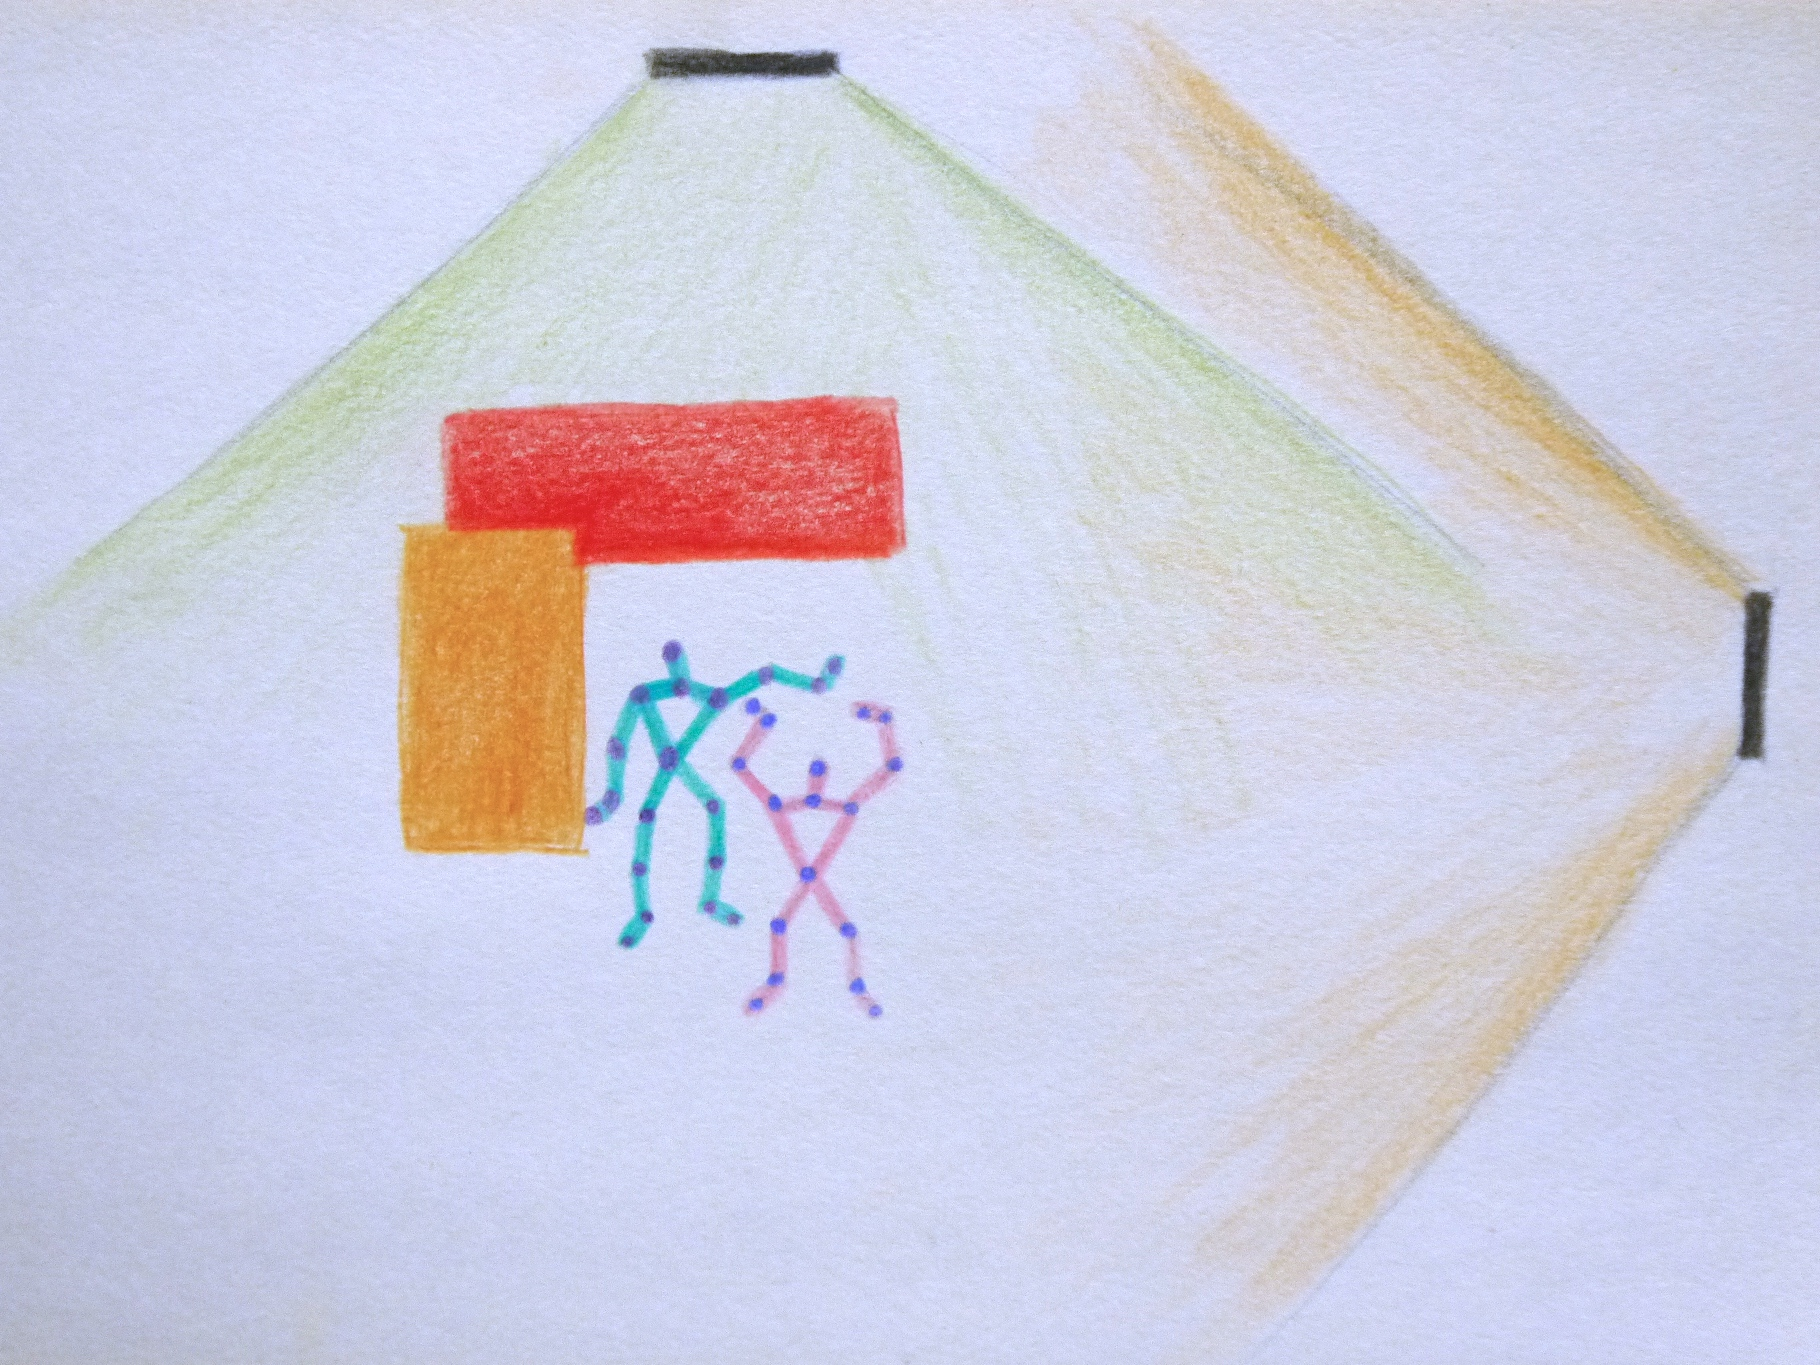
\includegraphics[width=0.8\linewidth]{occlusion}
\end{figure}
\end{frame}

\begin{frame}
\frametitle{What is Kinect?}
A low-cost sensor for motion capturing and tracking
\begin{itemize}
	\item Infrared
	\item RGB
	\item Depth
	\item Skeleton
	\item Others...
\end{itemize}
\begin{figure}
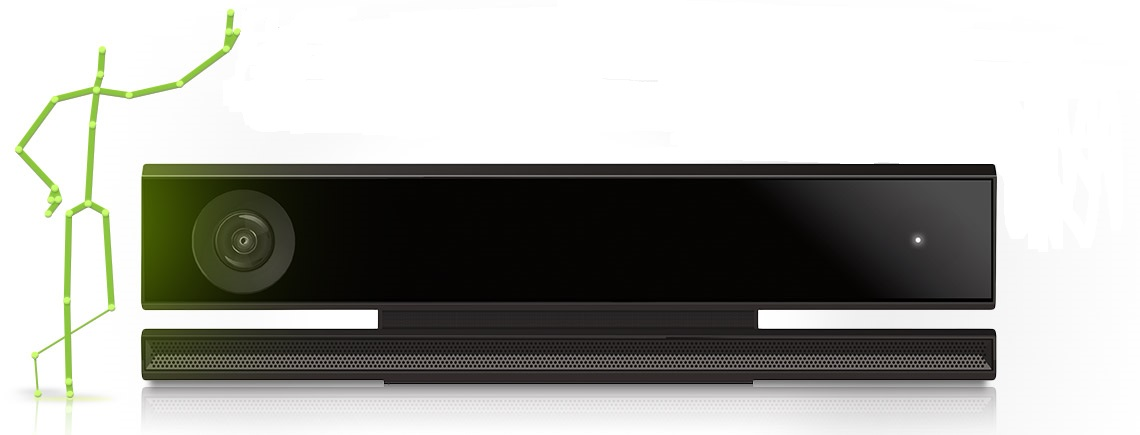
\includegraphics[width=0.8\linewidth]{kinect}
\end{figure}
\end{frame}

\begin{frame}
\frametitle{Infrared}
\begin{figure}
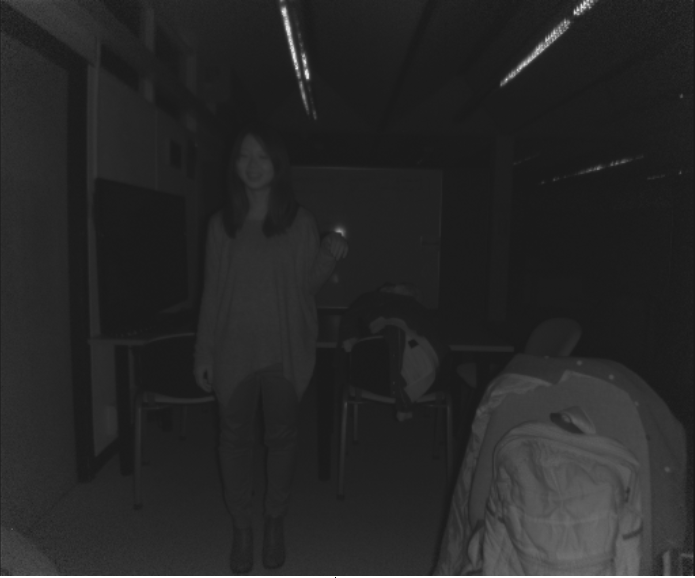
\includegraphics[width=0.7\linewidth]{infrared}
\end{figure}
\end{frame}

\begin{frame}
\frametitle{RGB}
\begin{figure}
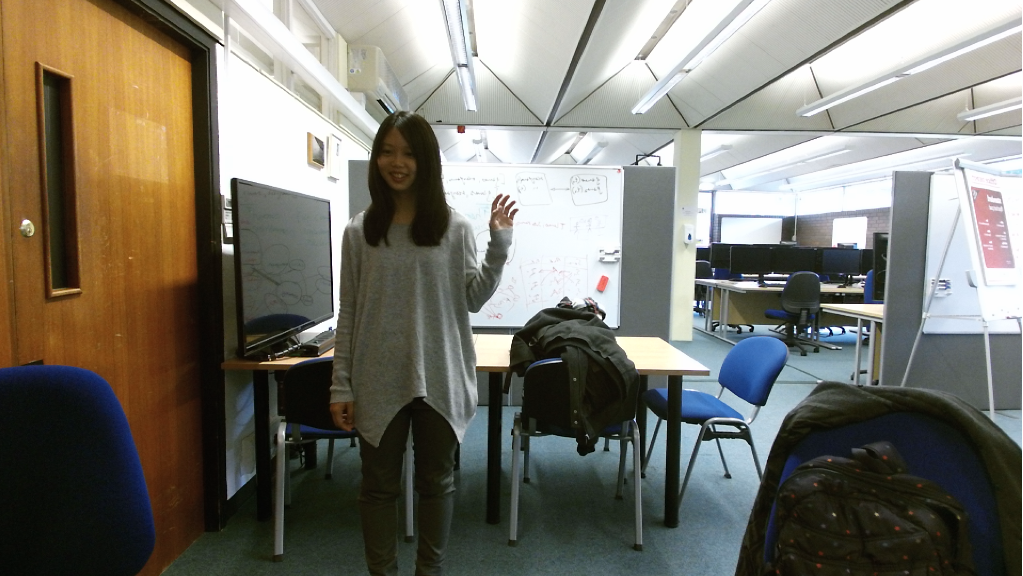
\includegraphics[width=0.7\linewidth]{color}
\end{figure}
\end{frame}

\begin{frame}
\frametitle{Depth}
\begin{figure}
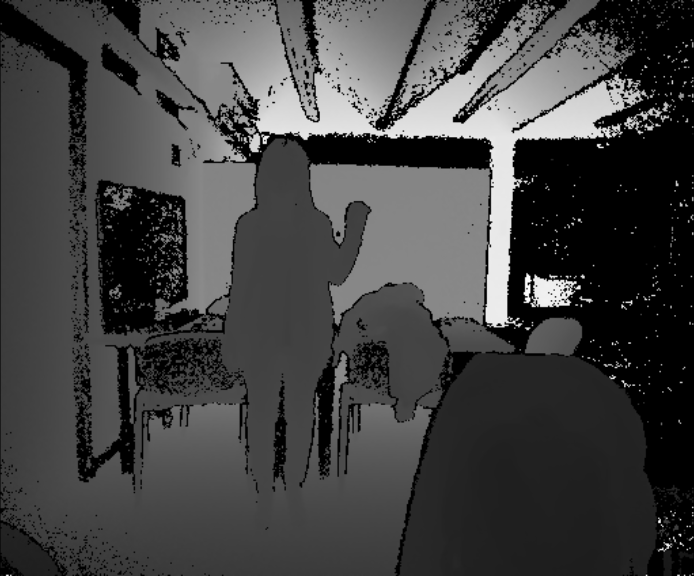
\includegraphics[width=0.7\linewidth]{depth}
\end{figure}
\end{frame}

\begin{frame}
\frametitle{Skeleton}
\begin{figure}
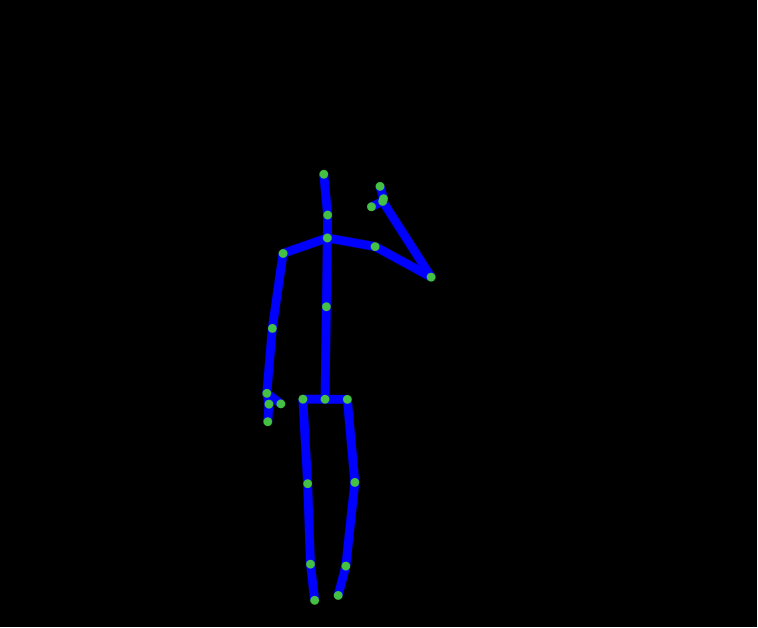
\includegraphics[width=0.7\linewidth]{skeleton}
\end{figure}
\end{frame}

\begin{frame}
\frametitle{Why use multiple Kinect?}
\begin{columns}[c]
\column{.45\textwidth}
\begin{itemize}
	\item Resolve the problem of occlusion
	\item Reconstruct 3D human models
	\item Human activity monitoring and prediction
\end{itemize}
\column{.5\textwidth}
\begin{figure}
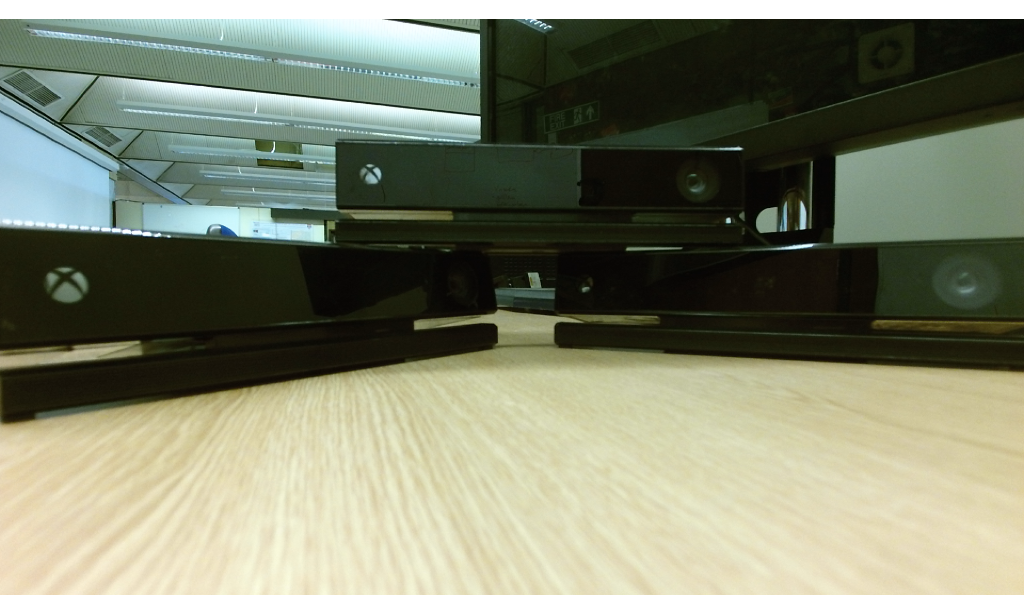
\includegraphics[width=0.8\linewidth]{multiple_kinects}
\newline{\tiny An image of multiple Kinects taken by another Kinect.\par}
\end{figure}
\end{columns}
\end{frame}

\begin{frame}
\frametitle{Things to consider...}
\begin{itemize}
	\item Calibration
	\item Occlusion objects
	\item Human interactions
	\item Illumination
	\item Simulated physical environments
\end{itemize}
\end{frame}

\section{Related Work}

\begin{frame}
\frametitle{What others have done?}
\begin{itemize}
	\item Infrared
	\item RGB
	\item Depth
\end{itemize}
\end{frame}

% \begin{frame}
% \frametitle{Infrared}
% \Huge{\centerline{TODO}}
% \end{frame}

\begin{frame}
\frametitle{RGB}
\begin{block}{Normalization}
Paper: Color transfer between images \cite{color_transfer}
\end{block}

\begin{block}{Color histogram}
Paper: A color histogram based people tracking system \cite{color_histogram}
\end{block}

\begin{block}{Histogram of gradients (HOG)}
Paper: Histograms of oriented gradients for human detection \cite{hog}
\end{block}

\begin{block}{Scale-invariant feature transform (SIFT)}
Paper: Distinctive Image Features from Scale-Invariant Keypoints \cite{sift}
\end{block}
\end{frame}

\begin{frame}
\frametitle{Depth}
Paper: Human Detection Using Depth Information by Kinect \cite{detection_depth}
\begin{itemize}
	\item 2D chamfer distance matching
	\item 3D model fitting
	\item Extract whole body contours
	\item Movement-based tracking
\end{itemize}
Paper: Tracking people within groups using RGB-D data \cite{rgbd}
\begin{itemize}
	\item sub-clustering
\end{itemize}
\end{frame}

\section{Current Approach}

\begin{frame}
\frametitle{What am I going to do?}
\begin{columns}[c]
\column{.45\textwidth}
\begin{itemize}
	\item Kinect calibration
	\item Gather user footage
	\item Track one person across different views
	\item Track one person with occlusion objects
	\item Track up to six users
	\item Test in various environments
\end{itemize}
\column{.5\textwidth}
\begin{figure}

\includegraphics[width=0.8\linewidth]{checklist}
\newline{\tiny AJ Cann, ``Feedback checklist'' August 22, 2013 via Flickr, Creative Commons Attribution.\par}
\end{figure}
\end{columns}
\end{frame}

\begin{frame}
\frametitle{Evaluation}
\begin{columns}[c]
\column{.45\textwidth}
\begin{itemize}
	\item Kinect footage
	\item Quantitative
\end{itemize}
\column{.5\textwidth}
\begin{figure}
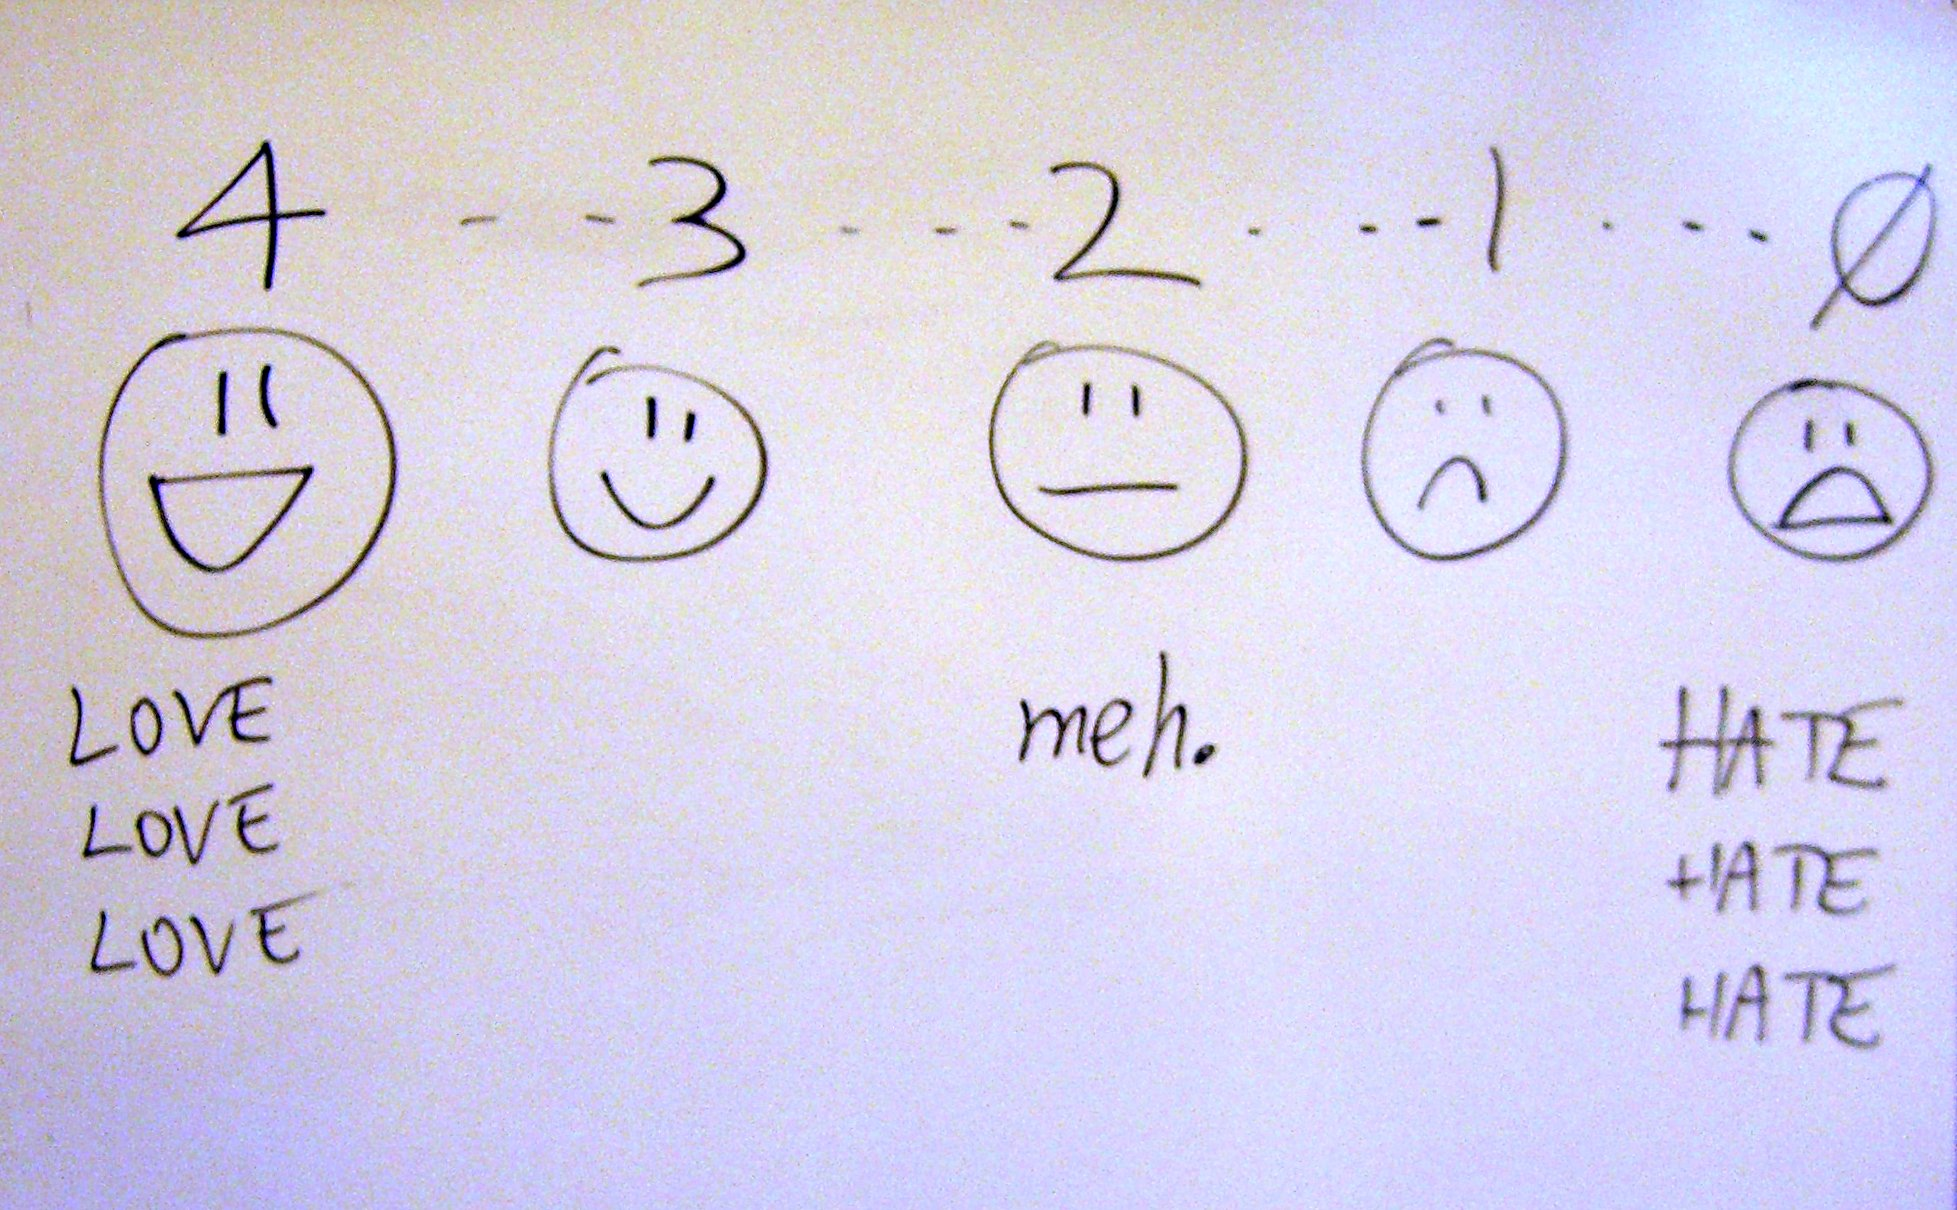
\includegraphics[width=0.8\linewidth]{evaluation}
\newline{\tiny billsoPHOTO, ``Evaluation scale'' December 10, 2009 via Flickr, Creative Commons Attribution.\par}
\end{figure}
\end{columns}
\end{frame}

\begin{frame}
\frametitle{Challenges}
\begin{itemize}
	\item Kinect calibration
	\item Merge different views into a single view
	\item Reduce the noise in depth data
	\item Real-time tracking
\end{itemize}
\end{frame}

\begin{frame}
\frametitle{References}
\footnotesize{
\begin{thebibliography}{4}
\bibitem[1]{color_transfer} [1] Reinhard, E., Ashikhmin, M., Gooch, B., \& Shirley, P. (2001)
\newblock Color transfer between images
\newblock \emph{IEEE Computer graphics and applications} 21(5), 34-41.
\bibitem[2]{color_histogram} [2] Lu, W., \& Tan, Y.P. (2001)
\newblock A color histogram based people tracking system
\newblock \emph{IEEE International Symposium on Circuits and Systems} 2, 137-140.
\bibitem[3]{hog} [3] Dalal, N., \& Triggs, B. (2005)
\newblock Histograms of oriented gradients for human detection
\newblock \emph{IEEE Computer Society Conference on Computer Vision and Pattern Recognition} 1, 886-893.
\bibitem[4]{sift} [4] DLowe, D. G. (2004)
\newblock Distinctive image features from scale-invariant keypoints
\newblock \emph{International journal of computer vision} 60(2), 91-110.
\end{thebibliography}
}
\end{frame}

\begin{frame}
\frametitle{References}
\footnotesize{
\begin{thebibliography}{4}
\bibitem[5]{detection_depth} [5] Xia, L., Chen, C. C., \& Aggarwal, J. K. (2011)
\newblock Human detection using depth information by Kinect
\newblock \emph{IEEE Computer Society Conference on Computer Vision and Pattern Recognition}, 15-22.
\bibitem[6]{rgbd} [6] Munaro, M., Basso, F., \& Menegatti, E. (2012)
\newblock Tracking people within groups with RGB-D data
\newblock \emph{IEEE International Conference on Intelligent Robots and Systems}, 2101-2107.
\end{thebibliography}
}
\end{frame}

\begin{frame}
\Huge{\centerline{The End}}
\end{frame}

\end{document}